\documentclass[a4paper,11pt,twoside]{article}
\usepackage[utf8]{inputenc}	% Text coding
\usepackage[T1]{fontenc}
\usepackage{lmodern}
\usepackage[czech]{babel}
\usepackage{epsfig}
\usepackage{amsfonts,amsmath,amssymb}
\usepackage{graphicx}
\usepackage[unicode]{hyperref}
\usepackage{indentfirst}
\usepackage{fancyhdr}
\usepackage{xifthen}
\usepackage{amsthm,thmtools}
\usepackage{bold-extra}
\usepackage[dvipsnames]{xcolor}
\usepackage[subrefformat=simple,labelformat=simple]{subcaption} % Instead of subfigure
\usepackage{listings}
\usepackage{comment}
\usepackage{titlesec}
\usepackage{underscore}
\usepackage{makecell}       % Šířky čar v tabulkách
\usepackage{wrapfig}

% Page size
\addtolength{\topmargin}{-1.5cm} %\addtolength{\textheight}{-10cm}
\addtolength{\textwidth}{4cm} \addtolength{\textheight}{4cm} % Width and height of the text
\addtolength{\voffset}{-0.5cm} % Top margin
\addtolength{\hoffset}{-2cm}
\setlength{\headheight}{15pt}

\DeclareMathOperator{\e}{e}

\def\vector#1{\boldsymbol{#1}}								% Vector
\renewcommand{\d}{\mathrm{d}}
\newcommand{\derivative}[3][]{\ifthenelse{\isempty{#1}}	    % Normal derivative
	{\frac{\d{#2}}{\d{#3}}}
	{\frac{\d^{#1}{#2}}{\d{#3}^{#1}}}
}
\newcommand{\im}{\mathrm{i}}

\def\makematrix#1{\begin{pmatrix}#1\end{pmatrix}}       % Matrix
\def\abs#1{\left|#1\right|}
\def\probability#1{\mathrm{Pr}\left[#1\right]}
\def\expectation#1{\mathrm{E}\left[#1\right]}
\def\dispersion#1{\sigma_{#1}^{2}}

\def\code#1{\textnormal{\texttt{#1}}}
\def\file#1{\textnormal{\textbf{\texttt{#1}}}}
\def\ghfile#1#2{\textnormal{\textbf{\texttt{\href{https://github.com/PavelStransky/PCInPhysics2021/blob/main/#1#2}{#2}}}}}

\def\abbreviation#1{\textnormal{\textsc{#1}}}

\begin{document}

\section*{Domácí úkol na 24.3.2025}
\subsection*{Integrace Monte Carlo}
\begin{enumerate}
    \item
        Naprogramujte univerzální funkci na výpočet integrálů funkcí jedné proměnné pomocí metody Monte Carlo
        a vypočítejte následující určité integrály:
        \begin{align}
            I_{1}&=\int_{0}^{\sqrt{10}}\e^{-x}\sin{x}\,\d x\\
            I_{2}&=\int_{0}^{1}\frac{1}{\sqrt{1+\frac{1}{\sqrt{1+x^{3}}}}}\d x
        \end{align}

    \item
        Vytvořte program, který spočítá metodou Monte Carlo objem $d$-rozměrné jednotkové koule $V_{d}$.
        Vykreslete závislost $V_{d}$ na dimenzi $d$ pro $d=1,\dotsc,10$ včetně odhadu chyby.
        Pro jakou dimenzi $d$ bude $V_{d}$ největší?

    \item
        Napište program pro výpočet hodnoty následujícího $d$-rozměrného integrálu pro libovolnou dimenzi $d$:
        \begin{equation}
            I_{3}=\int_{x_{1}^2+\dotsc+x_{d}^2<1}\cos\left(\sum_{i=1}^{d}x_{i}\right)\d x_{1}\dotsm\d x_{d}
        \end{equation}

    \item \emph{Gaussovka na srdci:}
    Metodou Monte Carlo vypočítejte integrál dvourozměrné Gaussovské funkce
    \begin{equation}
        I_{\heartsuit}=\int_{\heartsuit}\frac{1}{2\pi}\e^{-\frac{1}{2}\left(x^{2}+y^{2}\right)}\d x\,\d y
    \end{equation}
    na oblasti ohraničené implicitně křivkou (obrázek):
    \begin{equation}
        \heartsuit: \left(x^2+y^2-1\right)^3-x^2y^3\leq0
    \end{equation}
    \begin{center}
        \centering
        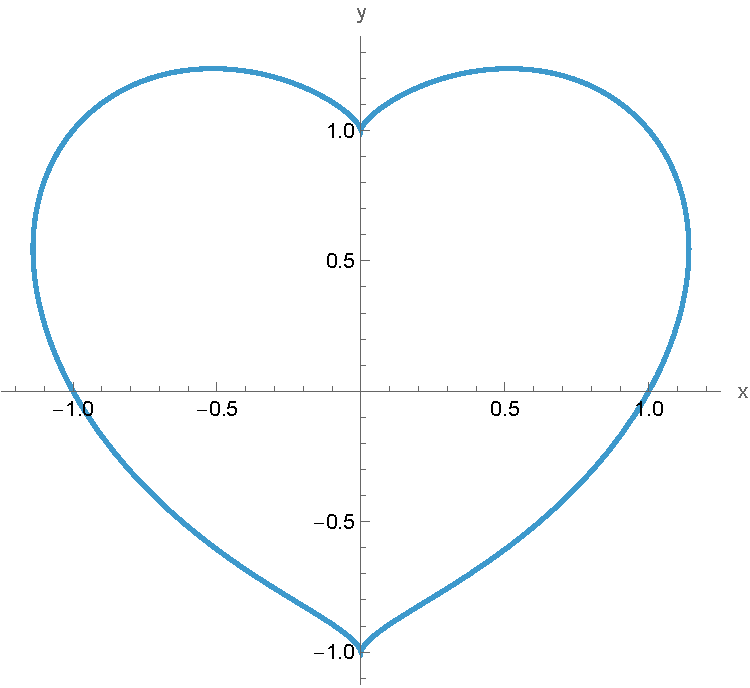
\includegraphics[width=0.5\linewidth]{heart.pdf}
    \end{center}
\end{enumerate}
\end{document}
